\chapter{研究问题和方法设计}
在本章,我们介绍研究的主体部分。我们首先展示我们的研究流程,再介绍研究仓库的选取,介绍四个基本的研究问题,介绍实验需要的自变量和因变量,并对数据的收集给出介绍,最后给出实验方法。

\section{研究流程}
图\ref{fig:image1},我们展示了本研究的流程图。

我们选定了十二个流行的Rust项目作为研究对象,如 egui、iced、nushell、clap 等。对于变更倾向,我们通过设定的规则遍历版本控制系统中所有commit,将所有commit划分为变更commit和非变更commit;对于错误倾向,我们通过版本控制系统找到所有的错误修复commit,然后通过预先定义的算法搜索错误引入commit。对于如上收集到的commit,我们通过求解语法树编辑距离算法,获得我们关注的变动部分。分别使用优势比分析和逻辑回归分析对变动部分进行分析,得出研究结果。

\begin{figure}[htbp]
  \centering
  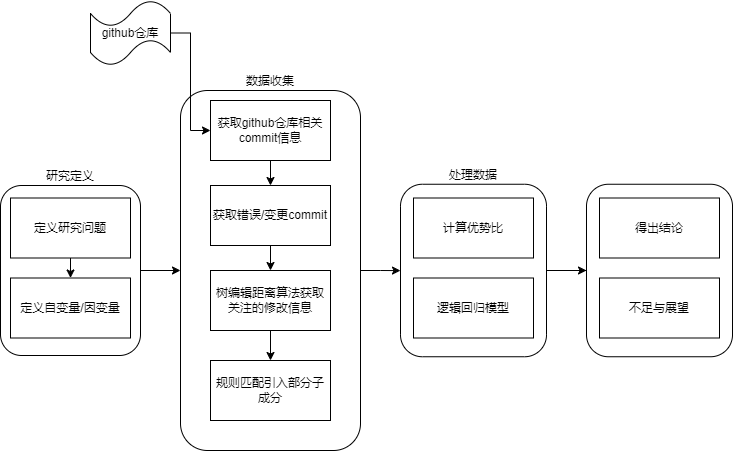
\includegraphics[width=0.8\textwidth]{picture/study_process.png}
  \caption{研究流程}
  \label{fig:image1}
\end{figure}

\section{研究仓库选取}  
这项研究的依据是十二个Rust系统的变更历史和问题跟踪系统。egui是一个用Rust编写的简单、快速、可移植的GUI库,主要用于开发即时模式的用户界面。它不依赖于本地操作系统提供的UI组件,因此可以轻松集成到各种应用程序中。iced是一个跨平台的GUI库,灵感来自于Elm语言的架构。它旨在创建纯Rust开发的简洁、反应灵敏的GUI应用程序,支持异步编程。nushell(通常称为nu)是一个新型的命令行shell,用Rust编写,结合了传统的shell功能和现代的数据处理能力。它支持表格数据的原生处理,使得对JSON、YAML等数据的处理更为直观和强大。clap是一个用于解析命令行参数和配置的库。它功能丰富,易于使用,支持自动生成帮助信息和错误消息,是创建命令行应用程序的理想选择。starship是一个快速、可定制的shell提示符,适用于多种shell(如bash、zsh、fish等)。它可以显示各种有用的信息,比如Git分支、Rust版本等,并且外观和功能高度可定制。TiKV是一个分布式键值数据库,最初由PingCAP公司开发,用于支持TiDB数据库的事务层。TiKV支持事务,提供强一致性保证,并通过Raft协议\cite{ongaro2014search}实现多副本数据复制。Firecracker是由Amazon Web Services开发的开源虚拟化技术,专为运行微虚拟机(microVMs)而设计,支持安全、高效地运行云原生服务器less计算工作负载。Tokio是一个Rust异步运行时,基于Rust的异步编程特性,广泛用于高性能网络服务和应用程序的开发。它支持异步I/O、任务调度等功能。Diem(前称Libra)是由Facebook启动的一个区块链项目,旨在创建一个稳定、无国界的数字货币。项目的目的是提供一种更安全、更低成本的支付方式。Vaultwarden是一个轻量级的Bitwarden密码管理服务的开源实现。它允许用户自行托管自己的密码库,而无需依赖第三方服务。actix-web是一个功能强大、易于使用的异步Web框架,支持构建高性能的Web应用程序。它基于Actix actor框架和Tokio异步运行时。rome/tools 是 Rome 的工具集,主要用于前端开发,包括代码格式化、linting、打包等功能。Rome 旨在成为一个全面的前端工具链,使前端开发更加统一和高效。

我们选取上述仓库的原因有如下几点:
\begin{enumerate}
    \item 这些仓库都是用 Rust 编程语言编写的,体现出了 Rust 在多种领域内的实际应用,包括 GUI 开发、命令行工具、网络编程、虚拟化技术、分布式系统等各种领域。
    \item 这些仓库都是在github中十分活跃,拥有很高的star数,受rust开发者广泛关注。
    \item 这些仓库的开发严格遵守开发规范,如pr、merge等行为有严格的规范,这样可以提高我们统计的准确性,减少因为开发者不规范导致的噪声。
\end{enumerate}

我们通过上述的仓库,采用预先设计的方法,进行实验数据的获取,并对获取实验数据进行分析,得到实验结论,并针对实验结论进行一定的分析。

以错误倾向为例,我们首先使用python脚本进行仓库的获取,然后从仓库的issue中找出特定标签的commit,通过我们设计的定义,找出引入这些错误的commit,使用工具获取这些commit中新引入的语法项以及语法项具体子成分,与其他非引入错误的commit进行对比,获得实验结论并对其分析讨论。

另外,我们在这里给出仓库的一些基本信息。

表\ref{tab:repo-info}给出了仓库的一些基本信息,commit表示仓库中commit的数量,Issue表示仓库主页issue的数目,GitHub Issue 是 GitHub 项目中用于追踪和讨论项目相关问题的功能。它可以被用来报告 bug、请求新功能、或者提出项目中的其他任务和问题。
\begin{table}[ht]
	\centering
        \caption{研究仓库信息}
	\begin{tabular}{ccccc}
        \toprule
		\textbf{repos}                             & \textbf{commit(个)} & \textbf{issue(个)} & \textbf{code line(行)} & \textbf{文件个数(个)} \\
        \midrule
		tikv/tikv                         & 7499   & 3567  & 446921    & 1183     \\
		nushell/nushell                   & 7994   & 3527  & 178342    & 1127     \\
		rome/tools                        & 4309   & 1353  & 247459    & 1262     \\
		iced-rs/iced                      & 3923   & 695   & 45819     & 323      \\
		  actix/actix-web                 & 4467   & 1389  & 52536     & 286      \\
		  firecracker-microvm/firecracker & 5898   & 1294  & 67816     & 276      \\
		  dani-garcia/vaultwarden         & 2649   & 1904  & 21301     & 52       \\
		  diem/diem                       & 9840   & 1060  & 323752    & 1730     \\
		tokio-rs/tokio                  & 3603   & 1801  & 79468     & 693      \\
		  clap-rs/clap                    & 7761   & 1671  & 52983     & 330      \\
		emilk/egui                        & 2754   & 861   & 56286     & 231      \\
		starship/starship                 & 2973   & 1501  & 35054     & 204  \\
        \bottomrule
	\end{tabular}
	\label{tab:repo-info}
\end{table}

表\ref{tab:bug-introduce-info}介绍了错误引入相关研究的信息,由于Rust版本变更十分漫长,过于旧的版本,不再具备参考价值,所以我们选取的是各仓库2021年之后的commit信息。

\begin{table}[ht]
	\centering
        \caption{错误引入信息}
	\begin{tabular}{ccc}
        \toprule
		\textbf{repos}                             & \textbf{错误引入commit(个)} & \textbf{非错误引入commit(个)} \\
        \midrule
		tikv/tikv                         & 649        & 1385        \\
		nushell/nushell                   & 704        & 4411        \\
		rome/tools                        & 334        & 1966        \\
		iced-rs/iced                      & 70         & 2278        \\
		  actix/actix-web                 & 50         & 891         \\
		  firecracker-microvm/firecracker & 18         & 2632        \\
		  dani-garcia/vaultwarden         & 42         & 1169        \\
		  diem/diem                       & 19         & 2430        \\
		tokio-rs/tokio                    & 126        & 1169        \\
		  alacritty/alacritty             & 98         & 425         \\
		  clap-rs/clap                    & 136        & 3811        \\
		emilk/egui                        & 250        & 1646        \\
		starship/starship                 & 106        & 1620 \\
        \bottomrule
	\end{tabular}
	\label{tab:bug-introduce-info}
\end{table}

\section{研究定义}
\subsection{研究问题}
为了研究Rust 语法结构与变更及错误倾向性的关系,我们设计了如下几个研究问题,试图通过下面的问题来得到一定的结论,这些问题由浅入深地研究了我们的研究主题。
\begin{itemize}
    \item RQ1: 不同语法项与变更倾向性之间的关系是什么?在这里我们研究各种语法项是不是容易发生变更,不同语法项之间会不会有哪些更容易发生变更。
    - H01: 某些语法项比其他语法项更易变更。
    \item RQ2: 特定语法项中的引入类型与变更倾向性之间的关系是什么?我们进一步观察每个语法项内部的各个子成分对于变更倾向的影响。
    - H02: 某种语法结构中的特定引入类型比其他类型更易变更。
    \item RQ3: 不同语法项与错误倾向性之间的关系是什么?在这里我们研究各种语法项是不是容易引入错误,不同语法项之间会不会有哪些明显更容易引发错误。
    - H03: 某些语法项比其他语法项更易出现错误。
    \item RQ4: 特定语法项中的引入类型与错误倾向性之间的关系是什么?我们进一步观察每个语法项内部的各个子成分对于引入错误的影响。
      - H04: 某种语法结构中的特定引入类型比其他类型更易出现错误。
\end{itemize}

\subsection{自变量}
Rust Reference 是 Rust 编程语言的官方参考手册,它提供了详尽的说明和解释,涵盖 Rust 语言的所有语法和特性。在我们的实验中,我们从该参考手册选取了items作为研究对象:

\begin{itemize}
    \item Module (mod): 用于组织代码,将功能相关的代码块分组在一起。模块可以嵌套,有助于创建清晰的代码结构。
    \item ExternCrate: 在2018 edition之前,用于声明外部库的依赖关系。在Rust 2018 edition中,这一语法项通常不再需要,因为Cargo.toml文件已足够处理外部依赖。
    \item ConstantItem (const): 用于定义常量,这些常量在编译时就已确定值,且值不可变。
    \item MacroInvocationSemi: 指在代码中调用宏时用分号结尾的语法结构,常用于执行宏而不返回值。
    \item MacroRulesDefinition (macro\_rules!): 定义宏的语法结构,允许编写可重复使用的代码模式。
    \item ExternBlock (extern): 用于声明外部函数接口,常用于与C语言等其他语言的互操作。
    \item Struct: 定义一个结构体,用于创建带有多个可能不同类型的字段的数据类型。
    \item Union: 类似结构体,但所有字段共享内存。常用于底层系统编程中的内存节省和特定类型操作。
    \item Enumeration (enum): 用于定义一个可以是几种不同值中的一个的类型。
    \item TypeAlias (type): 用于给现有的类型创建别名,有助于简化复杂类型的使用或提高代码的可读性。
    \item Function (fn): 定义一个函数,是执行代码的基本单元。
    \item Implementation (impl): 用于给结构体、枚举或特性实现具体的方法和关联函数。
    \item Trait: 定义一组方法(可以包含实现),其他类型可以实现(impl)这些方法,实现接口编程。
    \item AssociatedType: 在trait定义内部定义的类型,使得trait可以在不同的实现中具有不同的类型。
    \item UseDeclaration (use): 用于引入作用域中的路径,简化类型或函数的访问。
    \item StaticItem (static): 定义全局变量,这些变量在程序运行期间始终存在,与const的不同之处在于,static可以是可变的。
    \item GenericParams: 在定义函数、结构体、枚举、trait时,使用泛型参数使其可以适用于多种数据类型。
\end{itemize}
对于各语法项,我们选取了我们关注的一些语法成分,试图用模型衡量它们对于变更或错误引入倾向性的影响。下面是我们为各个语法项选取的子成分。
\begin{table}[tbp]
	\centering
        \caption{各个语法项关注的子成分}
	\begin{tabular}{cccccc}
        \toprule
		\textbf{语法项}            & \textbf{子成分1}                & \textbf{子成分2}         & \textbf{子成分3}         & \textbf{子成分4}         & \textbf{子成分5}        \\
        \midrule
		ExternCrate    & CrateRef            & AsClause     &              &              &             \\
		ConstantItem   & type                & expression   &              &              &             \\
		ExternBlock    & unsafe              & Abi          & Visibility   &              &             \\
		Struct         & visibility\_modifier & type         &              &              &             \\
		Union          & visibility\_modifier & type         &              &              &             \\
		Enumeration    & visibility\_modifier & expression   & type         &              &             \\
		TypeAlias      & lifetime            & trait\_bounds &              &              &             \\
		Function       & function\_modifiers  & parameters   & lifetime     & trait\_bounds & return\_type \\
		Implementation & unsafe              & lifetime     & trait\_bounds & TypePath     &             \\
		Trait          & unsafe              & lifetime     & trait\_bounds &              &             \\
		StaticItem     & mut                 & type         & expression   &              &             \\
		GenericParams  & LifetimeParam       & ConstParam   & TypeParam    &              &          \\
        \bottomrule
	\end{tabular}
	\label{tab:components}
\end{table}

如表2-1,我们展示了在探讨语法项子成分对变更和错误倾向性的影响时我们所关注的语法项的子成分。在这里,我们介绍一下我们关注他们的理由。
\begin{itemize}
    \item ExternCrate(CrateRef, AsClause): 我们关注CrateRef因为它直接指向外部库的引用,这是理解依赖管理的关键;而AsClause则使我们能够观察到命名空间的自定义使用,影响代码的可读性和可维护性。
    \item ConstantItem(type, expression): 我们关注type是因为它定义了常量的数据类型,直接影响程序的类型安全;expression则体现了常量的计算逻辑,可能是错误和性能问题的源头。
    \item ExternBlock(unsafe, Abi, Visibility): 我们关注unsafe以理解潜在的安全风险点;Abi指明了与外部代码的接口,关键于跨语言调用的稳定性;Visibility决定了访问级别,影响模块之间的耦合度。
    \item Struct(visibility\_modifier, type): 我们关注visibility\_modifier来分析结构体的可访问性,这直接影响模块的封装性;type则定义了结构体的数据类型,是理解数据组织的基础。
    \item Enumeration(visibility\_modifier, expression, type): 我们关注visibility\_modifier以审视枚举的公开级别;expression和type则共同定义了枚举的值和类型,关键于程序的逻辑分支处理。
    \item TypeAlias(lifetime, trait\_bounds): 我们关注lifetime以评估类型别名在生命周期管理中的作用;trait\_bounds则揭示了类型约束,对理解类型的行为和兼容性至关重要。
    \item Function(function\_modifiers, parameters, lifetime, trait\_bounds, return\_type): 我们关注function\_modifiers来了解函数的特殊属性如异步或不可变性;parameters, lifetime, trait\_bounds, 和return\_type共同定义了函数的接口和行为,是理解函数设计和使用的核心。
    \item Implementation(unsafe, lifetime, trait\_bounds, TypePath): 我们关注unsafe因为它表明代码中潜在的高风险区域;lifetime和trait\_bounds提供了实现细节的上下文,而TypePath则定位具体实现的结构或特性。
    \item Trait(unsafe, lifetime, trait\_bounds): 我们关注unsafe以识别特性中的安全漏洞;lifetime和trait\_bounds则是理解特性的行为限制和扩展性的关键。
    \item StaticItem(mut, type, expression): 我们关注mut以监控全局变量的可变性,这对并发编程至关重要;type和expression则分别定义了静态项的数据类型和初始化逻辑,直接关联到程序的运行时状态。
    \item GenericParams(LifetimeParam, ConstParam, TypeParam): 我们关注LifetimeParam以评估泛型在生命周期管理中的角色;ConstParam和TypeParam则分别揭示了泛型参数的常量性质和类型多样性,是泛型编程的基石。
\end{itemize}

对于RQ1和RQ3,我们统计每个commit中新增部分所属的item,定义为$A_{ic}$ commit $c$ 中统计到的item $i$ 的数量。对于RQ2和RQ4,我们统计到具体item下具体的子成分,定义$A{ijc}$ 为commit $c$ 中统计到的item $i$ 中的子成分 $j$ 的数量。

\subsection{因变量}
\label{sec:dependent-var}
因变量对应不同item或其子成分影响下commit发生的现象。

RQ1和RQ2 变更倾向指的是在一个commit中的所有文件中,是否存在某个文件发生了变更。变更被定义为从已有的代码变为新的代码,对应增删查改中的改。在进行源代码变更分析中,使用 tree-sitter-rust 来生成 Rust 语言的抽象语法树(AST)是研究的关键一环。tree-sitter-rust 是 tree-sitter 的一个针对 Rust 语言定制的模块,专门设计以解析 Rust 代码并生成遵循 Rust 语法规则的 AST。这一特性使得能够在语法层面上精确地分析代码变更,例如识别特定的语法结构在不同版本代码中的修改或替换。

通过比较连续两次提交的 AST 差异,本研究能够精确识别代码中的具体修改,并进一步分析这些修改对软件质量和功能的影响。

RQ3和RQ4 
在我的研究中,错误倾向性被定义为在代码提交(commit)过程中新引入部分倾向于引入错误。对于引入错误的代码,我们试图实现自动化的识别方法,我们认为错误的引入可以从错误的修复来获取,修复错误的部分必定与引入错误的部分有关联,基于这个思想,我们有了错误引入的定义:对于一个commit,如果存在后来修复错误的commit修改了它引入的部分,则认为该commit发生了错误引入。

\section{数据收集}
我们的研究主题是RUST语法结构与变更及错误倾向性关系,要想研究二者关系,首先要获取到语法结构与变更或错误对应的变量,在前一节我们已经给出了相关变量的定义。在这里,我们的工作重点就在于如何收集这些数据,下面我们介绍数据收集的各个环节。

\begin{minipage}{\textwidth}
\begin{parcolumns}{2}
\colchunk{
\floatname{listing}{代码示例}
\begin{lstlisting}[caption={简单的求和程序}, keepspaces=true, label={code1}]
// version1
fn sum(nums: &[i32])->i32 {
  let mut total = 0;
  for num in nums {
      total += num;
  }
  total
}

fn main() {
  let data = vec![1, 2];
  print!("{}", sum(&data));
} 
\end{lstlisting}
}

\colchunk{
\begin{lstlisting}[caption={简化过的求和程序}, keepspaces=true, label={code2}]
// version2
fn sum(nums: &[i32])->i32 {
  nums.iter().sum()
}

fn main() {
  let data = vec![1, 2, 3];
  print!("{}", sum(&data));
}
\end{lstlisting}
}

\colplacechunks
\end{parcolumns}
\end{minipage}

\subsection{收集错误修复commit}
我们实现了自动化的获取脚本,具体工作细节如下:首先定义github仓库以及各仓库相关的标签列表,借助github api从github根据标签爬取相关的commit hash,根据commit hash 获取每次commit中改动的后缀为.rs的文件,存放在文件中,再根据commit hash和文件名将文件前后的变更保存到一个目录中。

\subsection{获取每次commit新增部分}
\textit{difftastic}\footnote{\url{https://github.com/Wilfred/difftastic}} 工具是一个开源的源代码比较工具,与简单的文本比对不同,它借用tree-sitter将源代码解析为语法树,紧接着对语法树进行树编辑距离算法(核心是dijkstra算法)\cite{bille2005survey, pawlik2011rted, demaine2007optimal},得出前后改动的内容,这样的从语法层面的前后比较,比传统的文本比对更加精确,更加符合我们的需求。我们借用difftastic输出的中间结果,生成一个存放Hunk的向量,它代表左右子树各自新的内容,右子树新的内容即为我们关注的新增部分,如上面\ref{code1}和\ref{code2}代码段,version2中1,3,7,8行是新增行,他们要么是在version1中找不到相同的行(比如第一行注释行),要么有了新的修改(比如第7行的vec声明中多了一个元素)。

\subsection{获取每次commit删除部分}
同新增部分,我们借用difftastic输出的中间结果,生成一个存放Hunk的向量,左子树Hunk对应的内容,即删除部分。如上面\ref{code1}和\ref{code2}代码段,version1中的2,3,4,5,6行在version2中找不到相同的代码行,我们认为2,3,4,5,6行是被删除的行。

\subsection{收集错误引入commit}
为了准确地测量这种倾向性,我采用了一种基于历史数据的方法,通过分析开源项目的issue追踪系统中的标签来识别错误修复的提交(commit)。在算法\ref{algorithm1}中,我们简单描述了这个过程。具体来说,首先我们需要上面获取到的错误修复commit。一旦一个commit被标记为错误修复commit,将其标记为commit C。

为了确定哪些先前的提交可能引入了这些错误,我遍历了每个错误修复commit之前的所有普通commit。通过比较这些普通commit和commit C的代码变更部分,如果发现普通commit中的代码修改与commit C有交集,即这些修改出现在后来的错误修复提交中,那么这些普通commit被标记为错误引入commit。这种方法允许我们直接关联特定的代码修改与后续修复的错误,从而揭示代码变更的质量和风险。

此处我们简化了算法,在实际收集信息时,每个commit的情况会非常复杂,我们需要基于一定的策略过滤掉无关commit,过滤掉无关文件。对于每个commit而言,它们往往不止有一个文件,在上面的算法中我们均假设只有一个文件,但多文件也只是增加了写代码的难度,基本策略都是一致的。

我使用了tree-sitter-rust来生成Rust代码的抽象语法树(AST),从而在更细粒度上比较代码变更。通过AST,可以更精确地识别和分析哪些具体的语法结构变更可能与错误的引入有关。这种基于AST的分析方法不仅提高了识别错误倾向的准确性,也增强了对代码变更影响的理解。

在实际操作中,我对多个开源Rust项目的历史提交数据进行了此类分析。这包括从项目的Git仓库中提取所有commit记录,然后使用自动化脚本标记含有错误的commit,并追溯可能引入错误的普通commit。通过这种方法,我能够收集到大量数据,这些数据不仅支持了对错误引入模式的深入分析,也为理解编码实践中的常见问题提供了实证基础。

\begin{algorithm}
\caption{搜索错误引入commit}
\label{algorithm1}
\begin{algorithmic}[1]
\State $\text{commit\_map} \gets \text{HashMap<Commit, Set<Commit>>}$
\ForAll{$C \in \text{Commits}$}
    \State $B0, B0' \gets \text{parse}(C)$
    \ForAll{$C' \in \text{Commits before } C$}
        \State $B1, B1' \gets \text{parse}(C')$
        \State $A \gets \text{get_addition}(B1, B1')$
        \State $D \gets \text{get_deletion}(B0, B0')$
        \State $res \gets \text{has\_intersection}(B1', B0, A, D)$
        \If{$res = 1$}
            \State $\text{commit\_map.add}(C, C')$
        \EndIf
    \EndFor
\EndFor
\State \Return $\text{commit\_map}$
\end{algorithmic}
\end{algorithm}

\subsection{获取新引入item以及其组成部分}
通过difftastic工具获取新引入的tree-sitter语法树节点,这个节点一般是叶子结点,即表示源代码中具体某个token的节点,比如函数中的fn、int32类型、funcname。我们找到该节点,然后在语法树中从叶子结点到根节点向上搜索,选取第一个遇到的item为新引入item,如果该item是另一个item的子节点,只选取最近的祖先item作为新引入节点。通过编写预定的规则,去匹配目标的component,编写的算法可以匹配大部分情况,准确性很高。

如算法\ref{algorithm2}所示,我们首先定义一个遍历栈,从叶子结点开始向根节点遍历,每次把途经节点加入到遍历栈中,一旦我们的遍历找到类型为语法项的节点,我们停止遍历,此时栈中的内容即为语法项到具体改动叶子节点的路径,我们通过将此路径与预先定义的规则相匹配,即可找到本次item改动的具体类型。其中,ITEM2COMPONENTS是我们定义的一个哈希表,它的键是语法树节点,值是可能存在我们所关注子成分的子节点,这样我们从语法项节点向叶子节点的方向进行搜索,每次查询当前节点是否在父亲节点关注的子节点中,如果在,则继续遍历;如果发现不在,则说明后面的内容没有我们所关注的子节点。

\begin{algorithm}
\caption{获取语法项对应组件的函数}
\label{algorithm2}
\begin{algorithmic}[1]
\Function{GetComponentOfItemNode}{$\text{cursor1}: \text{TreeCursor}$}
    \State $\text{cursor} \gets \text{clone}(\text{cursor1})$
    \State $\text{travel\_stack} \gets \text{empty stack}$
    \State $\text{item\_string} \gets \text{empty string}$
    \While{$\text{not at root}$}
        \If{$\text{cursor node is syntax item}$}
            \State $\text{item\_string} \gets \text{cursor node kind}$
            \State $\textbf{break}$
        \EndIf
        \State $\text{push cursor node to travel\_stack}$
        \State $\text{move cursor to parent}$
    \EndWhile
    \State $\text{map} \gets \text{ITEM2COMPONENTS[item\_string]}$
    \For{$\text{node} \gets \text{travel\_stack.reverse()}$}
        \If{$\text{map contains key(node.kind)}$}
            \If{$\text{map[node.kind].kind} == \text{ChilditemKind::Container}$}
                \State $\text{map} \gets \text{ITEM2COMPONENTS[node.kind]}$
            \Else
                \State \Return $\text{node}, \text{map[node.kind].name}$
            \EndIf
        \Else
            \State \Return $\text{None}$
        \EndIf
    \EndFor
    \State \Return $\text{None}$
\EndFunction
\end{algorithmic}
\end{algorithm}

\section{数据分析}
RQ1和RQ3:我们为了研究commit中的变更和错误引入是否跟某些语法item的引入有关,我们计算了优势比(odds ratio\cite{bland2000odds}),他表示一个事件发生的可能性,比如说变更,OR被定义为一个样本中事件发生的几率p与另一个样本中发生的几率q的比值:OR = p/(1-p) / q/(1-q)。比值比为1表示两个样本中事件发生的可能性相同。OR > 1 表示事件在第一个样本中(含有某些语法item的实验组commit)更有可能发生,而OR < 1 表示相反的情况(不含有某些语法item的对照组commit)。

RQ2和RQ4:逻辑回归可以用于进行影响力分析,尤其是当你想了解哪些变量对某个具体事件(通常是二元的)的发生有显著影响时。我们为了研究语法item的特定子成分变更与错误和变更之间的关系,在这里使用逻辑回归模型进行一个统计分析,统计特定语法item的各种子成分对于变更/引入错误是否有显著影响。\cite{stoltzfus2011logistic}

在逻辑回归模型中,因变量通常是二元变量,因此它假定两个值{0,1},例如,变更与否。多变量逻辑回归基于如下的公式:

$π(X1, X2, ..., Xn) = \frac{e^{C0+C1·X1+...+Cn·Xn}} { 1 + e^{C0+C1·X1+...+Cn·Xn}}$

\begin{itemize}
    \item Xi是描述被建模现象的特征,在我们的案例中是参与第i种变更类型的item的数量。
    \item 0 ≤ π ≤ 1是逻辑回归曲线上的一个值。这个值越接近1表示发生变更的概率越高。
\end{itemize}